% System diagram for the VE paper. Source of the pipeline: docs/architecture-and-design.md,
% section "Components and trust boundaries". Compile with: tectonic system.tex
\documentclass[tikz,border=4pt]{standalone}
\usetikzlibrary{arrows.meta,positioning,fit}
\begin{document}
\sffamily\small
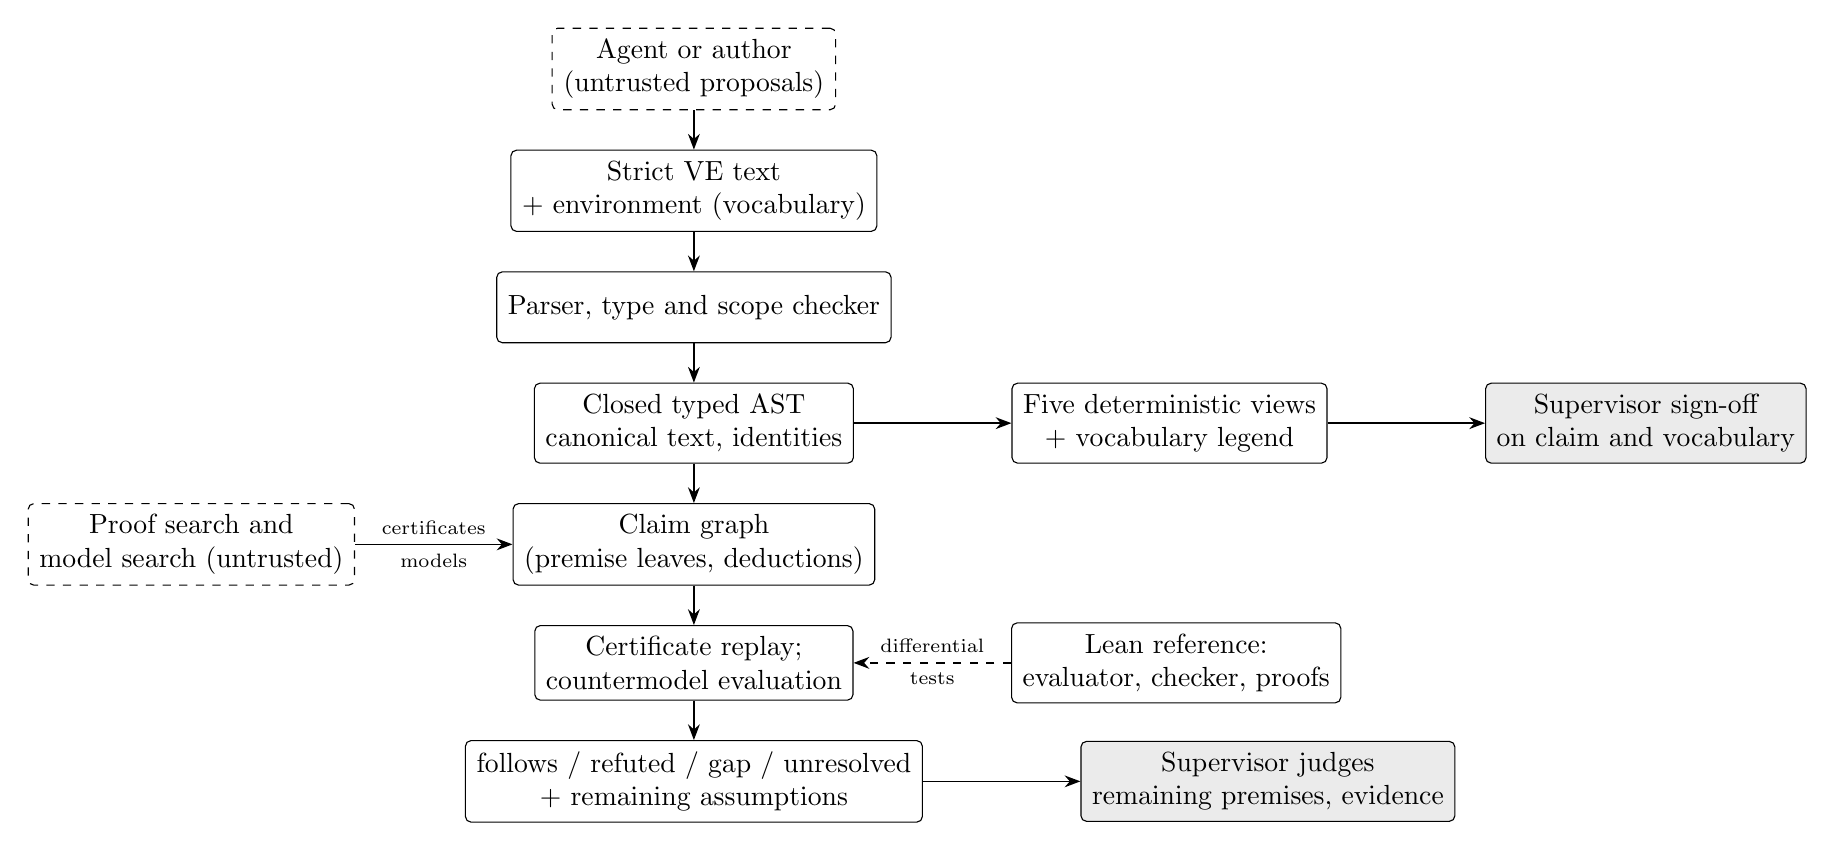
\begin{tikzpicture}[
  node distance=5mm and 20mm,
  box/.style={draw, rounded corners=2pt, align=center, inner sep=4pt, minimum width=36mm, minimum height=9mm},
  untrusted/.style={box, dashed},
  human/.style={box, fill=black!8},
  arr/.style={-{Stealth[length=2mm]}, semithick},
  note/.style={align=left, font=\scriptsize}
]
\node[untrusted] (agent) {Agent or author\\(untrusted proposals)};
\node[box, below=of agent] (src) {Strict VE text\\+ environment (vocabulary)};
\node[box, below=of src] (parse) {Parser, type and scope checker};
\node[box, below=of parse] (ast) {Closed typed AST\\canonical text, identities};
\node[box, right=of ast] (views) {Five deterministic views\\+ vocabulary legend};
\node[human, right=of views] (signoff) {Supervisor sign-off\\on claim and vocabulary};
\node[box, below=of ast] (graph) {Claim graph\\(premise leaves, deductions)};
\node[untrusted, left=of graph] (search) {Proof search and\\model search (untrusted)};
\node[box, below=of graph] (check) {Certificate replay;\\countermodel evaluation};
\node[box, below=of check] (result) {follows / refuted / gap / unresolved\\+ remaining assumptions};
\node[human, right=of result] (judge) {Supervisor judges\\remaining premises, evidence};
\node[box, right=of check] (lean) {Lean reference:\\evaluator, checker, proofs};
\draw[arr] (agent) -- (src);
\draw[arr] (src) -- (parse);
\draw[arr] (parse) -- (ast);
\draw[arr] (ast) -- (views);
\draw[arr] (views) -- (signoff);
\draw[arr] (ast) -- (graph);
\draw[arr] (search) -- node[above, note] {certificates} node[below, note] {models} (graph);
\draw[arr] (graph) -- (check);
\draw[arr] (check) -- (result);
\draw[arr] (result) -- (judge);
\draw[arr, dashed] (lean) -- node[above, note] {differential} node[below, note] {tests} (check);
\end{tikzpicture}
\end{document}
